\documentclass[border=4pt]{standalone}
\usepackage[T1]{fontenc}
\usepackage{newtxtext,newtxmath}
\usepackage{tikz}
\usetikzlibrary{arrows.meta,calc,positioning,shapes.geometric}
\definecolor{ink}{HTML}{24313E}
\definecolor{blue}{HTML}{4477AA}
\definecolor{teal}{HTML}{338899}
\definecolor{amber}{HTML}{BB7711}
\definecolor{red}{HTML}{AA4455}
\begin{document}
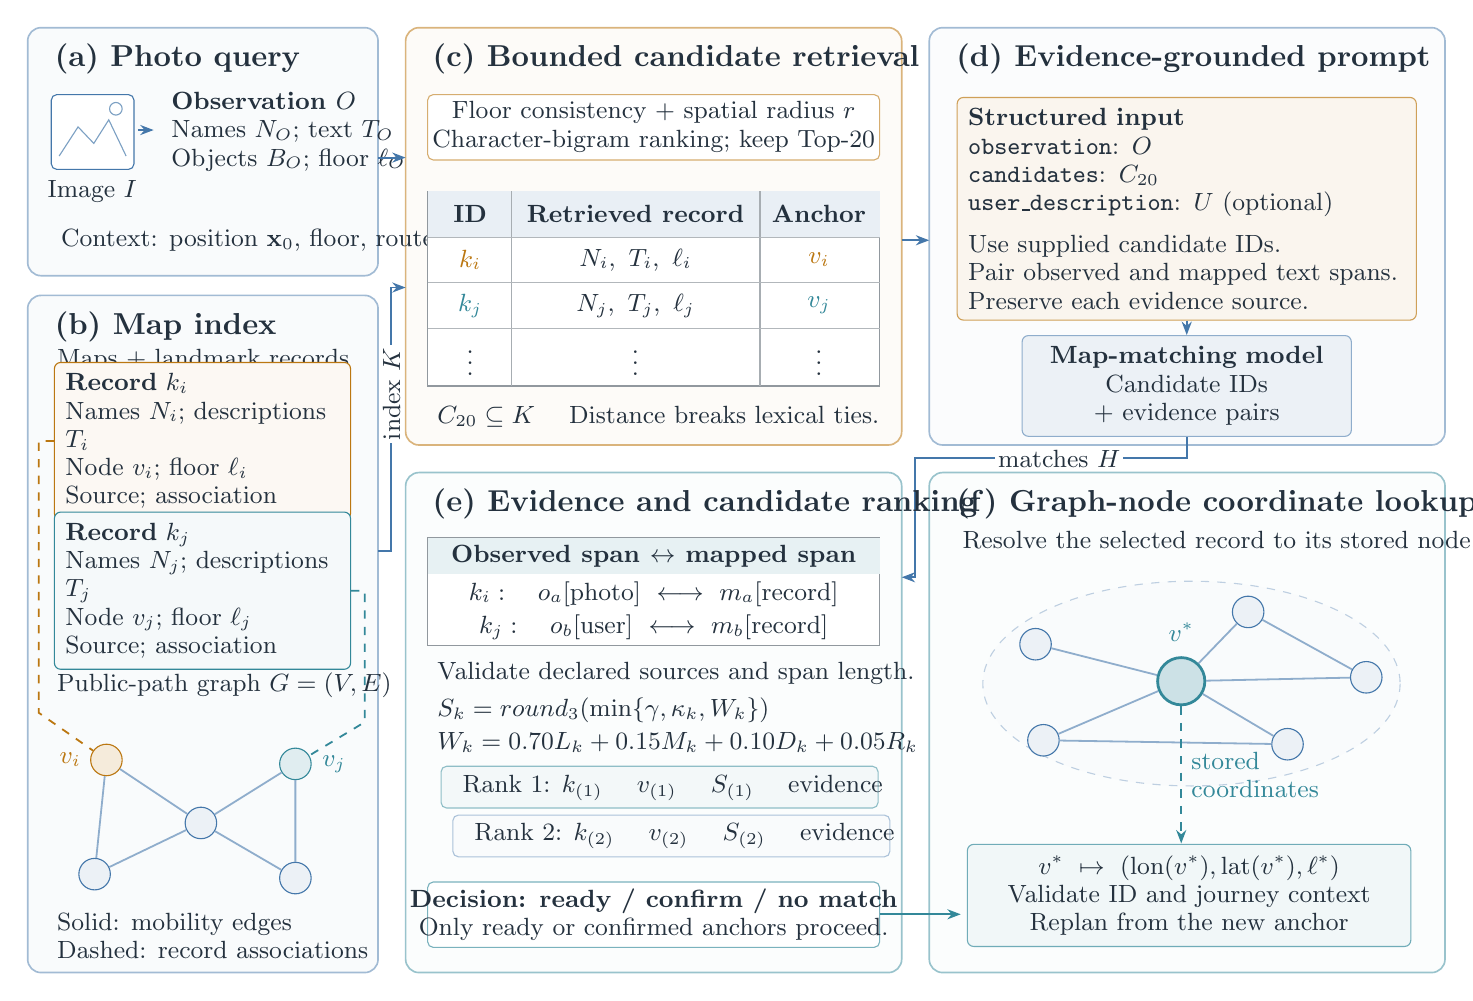
\begin{tikzpicture}[x=1cm,y=-1cm,text=ink,font=\fontsize{9}{10.5}\selectfont,
 arr/.style={-{Stealth[length=1.7mm]},line width=.7pt,draw=blue},
 link/.style={draw=blue!60,line width=.65pt},
 assoc/.style={draw=amber,dashed,line width=.65pt},
 panel/.style={rounded corners=1.7mm,line width=.6pt},
 title/.style={font=\fontsize{10.5}{12}\selectfont\bfseries,anchor=west},
 small/.style={font=\fontsize{8.7}{10.2}\selectfont},
 card/.style={draw=blue!60,fill=white,rounded corners=.8mm,align=left,inner sep=4pt,font=\fontsize{8.7}{10.2}\selectfont},
 vertex/.style={circle,draw=blue,fill=blue!10,minimum size=4mm,inner sep=0pt}]
\path[use as bounding box] (0,0) rectangle (18,12);
\draw[panel,draw=blue!50,fill=blue!3] (0,0) rectangle (4.45,3.15);
\draw[panel,draw=blue!50,fill=blue!3] (0,3.4) rectangle (4.45,12);
\draw[panel,draw=amber!55,fill=amber!3] (4.8,0) rectangle (11.1,5.3);
\draw[panel,draw=blue!50,fill=blue!2] (11.45,0) rectangle (18,5.3);
\draw[panel,draw=teal!50,fill=teal!2] (4.8,5.65) rectangle (11.1,12);
\draw[panel,draw=teal!50,fill=teal!2] (11.45,5.65) rectangle (18,12);

% Query representation: symbolic image and structured observation.
\node[title] at (.22,.4) {(a) Photo query};
\draw[draw=blue,fill=white,rounded corners=.7mm] (.3,.85) rectangle (1.35,1.8);
\draw[blue!70] (.4,1.63)--(.64,1.26)--(.84,1.47)--(1.03,1.17)--(1.25,1.63);
\draw[blue!70] (1.12,1.03) circle (.08);
\node[small] at (.82,2.08) {Image $I$};
\draw[arr] (1.4,1.3)--(1.6,1.3);
\node[small,anchor=west,align=left] at (1.7,1.32)
 {\textbf{Observation $O$}\\Names $N_O$; text $T_O$\\Objects $B_O$; floor $\ell_O$};
\node[small,anchor=west] at (.3,2.7) {Context: position $\mathbf{x}_0$, floor, route};
\draw[arr] (4.45,1.65)--(4.8,1.65);

% Stored records with explicit associations to mobility graph nodes.
\node[title] at (.22,3.8) {(b) Map index};
\node[small,anchor=west] at (.25,4.23) {Maps + landmark records};
\node[card,text width=3.48cm,draw=amber,fill=amber!5] (ki) at (2.22,5.25)
 {\textbf{Record $k_i$}\\Names $N_i$; descriptions $T_i$\\Node $v_i$; floor $\ell_i$\\Source; association};
\node[card,text width=3.48cm,draw=teal,fill=teal!5] (kj) at (2.22,7.15)
 {\textbf{Record $k_j$}\\Names $N_j$; descriptions $T_j$\\Node $v_j$; floor $\ell_j$\\Source; association};
\node[small,anchor=west] at (.25,8.35) {Public-path graph $G=(V,E)$};
\node[vertex,draw=amber,fill=amber!15] (vi) at (1.0,9.3) {};
\node[vertex,draw=teal,fill=teal!15] (vj) at (3.4,9.35) {};
\node[vertex] (va) at (2.2,10.1) {};
\node[vertex] (vb) at (.85,10.75) {};
\node[vertex] (vc) at (3.4,10.8) {};
\draw[link] (vi)--(va)--(vj); \draw[link] (vi)--(vb)--(va)--(vc)--(vj);
\node[small,anchor=east,text=amber] at (.8,9.3) {$v_i$};
\node[small,anchor=west,text=teal] at (3.62,9.35) {$v_j$};
\draw[assoc] (ki.west)--(.14,5.25)--(.14,8.7)--(vi);
\draw[assoc,teal] (kj.east)--(4.28,7.15)--(4.28,8.82)--(vj);
\node[small,anchor=west,align=left] at (.25,11.53) {Solid: mobility edges\\Dashed: record associations};
\draw[arr] (4.45,6.65)--(4.62,6.65)--(4.62,3.3)--(4.8,3.3);
\node[small,rotate=90,fill=white,inner sep=1pt] at (4.62,4.65) {index $K$};

% Real retrieval is bounded spatial/lexical search, not graph expansion.
\node[title] at (5.02,.4) {(c) Bounded candidate retrieval};
\draw[draw=amber!60,fill=white,rounded corners=.7mm] (5.08,.85) rectangle (10.82,1.68);
\node[small,align=center] at (7.95,1.26)
 {Floor consistency + spatial radius $r$\\Character-bigram ranking; keep Top-20};
\draw[draw=ink!50,fill=white] (5.08,2.08) rectangle (10.82,4.55);
\fill[blue!12] (5.08,2.08) rectangle (10.82,2.66);
\draw[ink!40] (6.15,2.08)--(6.15,4.55);
\draw[ink!40] (9.3,2.08)--(9.3,4.55);
\foreach \y in {2.66,3.24,3.82} {\draw[ink!35] (5.08,\y)--(10.82,\y);}
\node[small] at (5.62,2.37) {\textbf{ID}};
\node[small] at (7.72,2.37) {\textbf{Retrieved record}};
\node[small] at (10.05,2.37) {\textbf{Anchor}};
\node[small,text=amber] at (5.62,2.95) {$k_i$};
\node[small] at (7.72,2.95) {$N_i,\ T_i,\ \ell_i$};
\node[small,text=amber] at (10.05,2.95) {$v_i$};
\node[small,text=teal] at (5.62,3.53) {$k_j$};
\node[small] at (7.72,3.53) {$N_j,\ T_j,\ \ell_j$};
\node[small,text=teal] at (10.05,3.53) {$v_j$};
\node[small] at (5.62,4.16) {$\vdots$};
\node[small] at (7.72,4.16) {$\vdots$};
\node[small] at (10.05,4.16) {$\vdots$};
\node[small,anchor=west] at (5.08,4.94) {$C_{20}\subseteq K$ \quad Distance breaks lexical ties.};
\draw[arr] (11.1,2.7)--(11.45,2.7);

% The retrieved records become model context.
\node[title] at (11.67,.4) {(d) Evidence-grounded prompt};
\node[card,text width=5.55cm,draw=amber!70,fill=amber!7,minimum height=2.7cm] (prompt) at (14.72,2.3)
 {\textbf{Structured input}\\
 \texttt{observation}: $O$\\
 \texttt{candidates}: $C_{20}$\\
 \texttt{user\_description}: $U$ (optional)\\[5pt]
 Use supplied candidate IDs.\\
 Pair observed and mapped text spans.\\
 Preserve each evidence source.};
\node[card,text width=3.9cm,align=center,fill=blue!10] (model) at (14.72,4.55)
 {\textbf{Map-matching model}\\Candidate IDs + evidence pairs};
\draw[arr] (prompt)--(model);
\draw[arr] (model.south)--(14.72,5.47)--(11.27,5.47)--(11.27,6.98)--(11.1,6.98);
\node[small,fill=white,inner sep=1pt] at (13.1,5.47) {matches $H$};

% Evidence pairs and candidate pool, without invented numeric scores.
\node[title] at (5.02,6.05) {(e) Evidence and candidate ranking};
\draw[draw=ink!50,fill=white] (5.08,6.48) rectangle (10.82,7.85);
\fill[teal!12] (5.08,6.48) rectangle (10.82,6.94);
\node[small] at (7.95,6.71) {\textbf{Observed span $\leftrightarrow$ mapped span}};
\node[small] at (7.95,7.19) {$k_i:\quad o_a[\mathrm{photo}]\ \longleftrightarrow\ m_a[\mathrm{record}]$};
\node[small] at (7.95,7.62) {$k_j:\quad o_b[\mathrm{user}]\ \longleftrightarrow\ m_b[\mathrm{record}]$};
\node[small,anchor=west] at (5.08,8.2) {Validate declared sources and span length.};
\node[small,anchor=west] at (5.08,8.67)
 {$S_k=\operatorname{round}_3\!\left(\min\{\gamma,\kappa_k,W_k\}\right)$};
\node[small,anchor=west] at (5.08,9.08)
 {$W_k=0.70L_k+0.15M_k+0.10D_k+0.05R_k$};
\draw[draw=teal!55,fill=teal!6,rounded corners=.7mm] (5.25,9.38) rectangle (10.8,9.91);
\node[small,anchor=west] at (5.4,9.65) {Rank 1: $k_{(1)}$ \quad $v_{(1)}$ \quad $S_{(1)}$ \quad evidence};
\draw[draw=blue!45,fill=blue!3,rounded corners=.7mm] (5.4,10.0) rectangle (10.95,10.53);
\node[small,anchor=west] at (5.55,10.27) {Rank 2: $k_{(2)}$ \quad $v_{(2)}$ \quad $S_{(2)}$ \quad evidence};
\draw[draw=teal!65,fill=white,rounded corners=.7mm] (5.08,10.85) rectangle (10.82,11.68);
\node[small,align=center] at (7.95,11.26)
 {\textbf{Decision: ready / confirm / no match}\\Only ready or confirmed anchors proceed.};
\draw[arr,teal] (10.82,11.26)--(11.85,11.26);

% Stored graph coordinates, rather than generated positions.
\node[title] at (11.67,6.05) {(f) Graph-node coordinate lookup};
\node[small,anchor=west] at (11.75,6.5) {Resolve the selected record to its stored node.};
\draw[draw=blue!35,dashed,fill=blue!3] (14.78,8.33) ellipse (2.65 and 1.3);
\node[vertex] (g1) at (12.8,7.83) {};
\node[vertex] (g2) at (15.5,7.42) {};
\node[vertex] (g3) at (17.0,8.25) {};
\node[vertex] (g4) at (16.0,9.1) {};
\node[vertex] (g5) at (12.9,9.05) {};
\node[vertex,draw=teal,line width=1pt,fill=teal!25,minimum size=6mm] (star) at (14.65,8.3) {};
\draw[link] (g1)--(star)--(g2)--(g3)--(star)--(g4)--(g5)--(star);
\node[small,anchor=south,text=teal] at (14.65,7.92) {$v^*$};

\node[card,text width=5.35cm,draw=teal!70,fill=teal!7,minimum height=1.05cm,align=center] (lookup) at (14.75,11.02)
 {$v^*\mapsto(\mathrm{lon}(v^*),\mathrm{lat}(v^*),\ell^*)$\\Validate ID and journey context\\Replan from the new anchor};
\draw[arr,teal,dashed] (star.south)--node[right,small,align=left] {stored\\coordinates}(14.65,10.36);
\end{tikzpicture}
\end{document}
